\chapter{Psalm 49}

\begin{figure}
  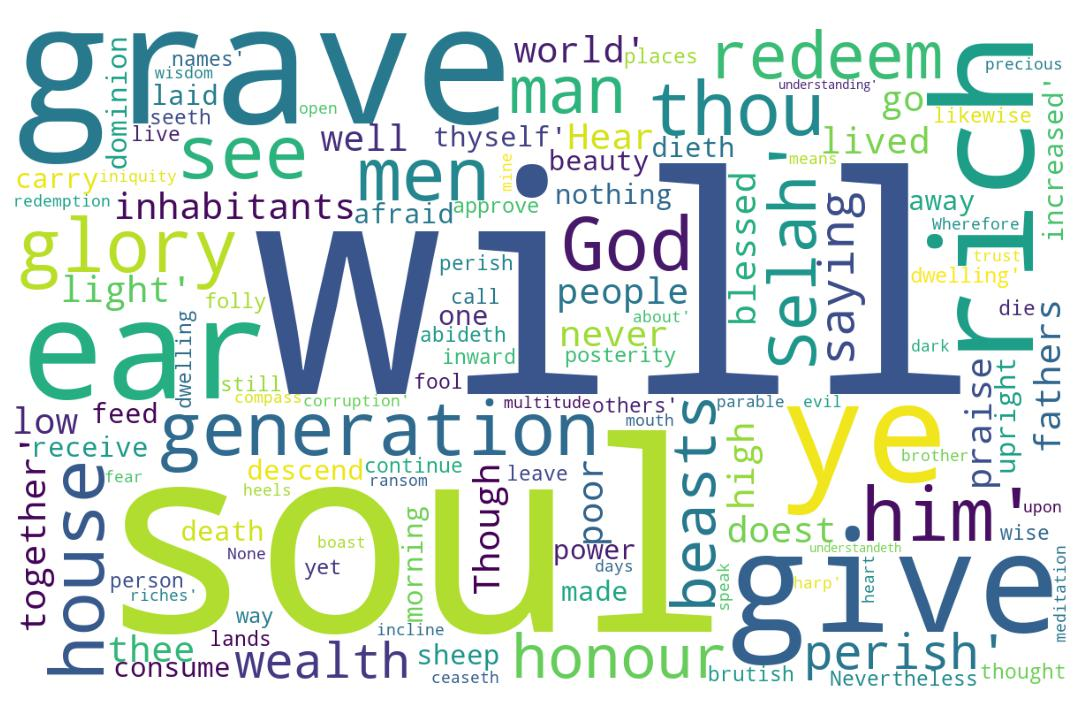
\includegraphics[width=\linewidth]{19OT-Psalms/Psalm49-WordCloud.jpg}
  \caption{Psalm 49 Word Cloud}
  \label{fig:Psalm 49 word Cloud}
\end{figure}

\marginpar{\scriptsize \centering \fcolorbox{bone}{lime}{\textbf{BIG PROBLEMS STILL REMAIN}}\\ (Psalm 49:1-20) \begin{compactenum}[I.][8]
    \item \textbf{Religious Conflict} \index[scripture]{Psalms!Psa 049:13} (Psa 49:13)
    \item \textbf{War} \index[scripture]{Psalms!Psa 049:13} (Psa 49:13)
    \item \textbf{Famine} \index[scripture]{Psalms!Psa 049:13} (Psa 49:13)
    \item \textbf{Sickness} \index[scripture]{Psalms!Psa 049:13} (Psa 49:13)
    \item \textbf{Death} \index[scripture]{Psalms!Psa 049:13} (Psa 49:13)
    \item \textbf{Natural Disasters} \index[scripture]{Psalms!Psa 049:13} (Psa 49:13)
    \item \textbf{Murder and Theft} \index[scripture]{Psalms!Psa 049:13} (Psa 49:13)
\end{compactenum}}


\marginpar{\scriptsize \centering \fcolorbox{bone}{yellow}{\textbf{THE BEASTS THAT PERISH}}\\ (Psalm 49:1-20) \begin{compactenum}[I.][8]
    \item The \textbf{Basic Problems}
    \item The \textbf{Brutish People}
    \item The \textbf{Broken ``Progress''}
    \item The \textbf{Bestowed Possessions}
    \item The \textbf{Beauty that Passes}
    \item The \textbf{Beasts that Perish}
\end{compactenum}}


    
%%%%%%%%%%%%%%%%%%%%%%%%%%%%%%%%%%%%%
%%%%%%%%%%%%%%%%%%%%%%%%%%%%%%%%%%%%%
\footnote{\textcolor[cmyk]{0.99998,1,0,0}{\hyperlink{TOC}{Return to end of Table of Contents.}}}\footnote{\href{https://audiobible.com/bible/psalms_49.html}{\textcolor[cmyk]{0.99998,1,0,0}{Psalms Audio}}}\textcolor[cmyk]{0.99998,1,0,0}{To the chief Musician, A Psalm for the sons of Korah.}\footnote{This is one of the ``orphan'' psalm, with no known author (anonymous), But, it is one of eleven psalms that were for the sons of Korah. (Psalm 42, 44, 45, 46, 47, 48, 49, 84, 85, 87, and 88). The sons of Korah descended from a father who perished under the wrath and curse of God because of his arrogance and pride.   As Korah was a Levite, grandson of Kohath, great-grandson of Levi, this only aggravated his fault, and typifies the sin of Israel, keepers of the oracles of God. \cite{Phillips2001ExploringPsalms1} The count of the psalms for the sons of Korah points to the number 11 as the number of the ``remnant'' as does Hebrews 11 which lists those distinct and select people know for the exercise of faith.}\\
\\
\textcolor[cmyk]{0.99998,1,0,0}{Hear this, all \emph{ye} people; give ear, all \emph{ye} inhabitants of the world:}
[2] \textcolor[cmyk]{0.99998,1,0,0}{Both low and high, rich and poor, together.}
[3] \textcolor[cmyk]{0.99998,1,0,0}{My mouth shall speak of wisdom; and the meditation of my heart \emph{shall} \emph{be} of \fcolorbox{bone}{MYGOLD}{understanding}.}
[4] \textcolor[cmyk]{0.99998,1,0,0}{I will incline mine ear to a parable: I will open my dark saying upon the harp.}
[5] \textcolor[cmyk]{0.99998,1,0,0}{Wherefore should I fear in the days of evil, \emph{when} the iniquity of my heels shall compass me about?}\footnote{The words ``heels'' is found four times in scripture, signifying that someone’s iniquities are following them. What we have done catches up with us (vs. 5). The steps we have stepped, out run us eventually because we step slower and slower. Sooner or later they compass us round about: \cite{Ruckman1992Psalms}
\begin{compactenum}
\item \textbf{Genesis 49:17} -- Dan shall be a serpent by the way, an adder in the path, that biteth the horse heels, so that his rider shall fall backward.
\item \textbf{Job 13:27} -- Thou puttest my feet also in the stocks, and lookest narrowly unto all my paths; thou settest a print upon the heels of my feet.
\item \textbf{Psalm 49:5} -- Wherefore should I fear in the days of evil, \emph{when} the iniquity of my heels shall compass me about?
\item \textbf{Jeremiah 13:22} -- And if thou say in thine heart, Wherefore come these things upon me? For the greatness of thine iniquity are thy skirts discovered, \emph{and} thy heels made bare.
\end{compactenum} }
[6] \textcolor[cmyk]{0.99998,1,0,0}{They that trust in \fcolorbox{bone}{bone}{their} wealth, and boast themselves in the multitude of \fcolorbox{bone}{bone}{their} riches;}\marginpar{\scriptsize \textcolor[rgb]{0.00,0.545,0.269}{$\rightarrow$``Their'' things: 
\begin{compactenum}
	\item their wealth [6, 10],
	\item their riches [6],
	\item their soul [7],
	\item their inward thought [11],
	\item their houses [11],
	\item their dwelling places [11],
	\item their lands [11],
	\item their names [11],
	\item their way [13],
	\item their folly [13],
	\item their posterity [13],
	\item their sayings [13],
	\item their beauty [15], and
	\item dwelling  [15].
\end{compactenum}}}
[7] \textcolor[cmyk]{0.99998,1,0,0}{None \emph{of} \emph{them} can by any means redeem his brother, nor give to God a ransom for him:}
[8] \textcolor[cmyk]{0.99998,1,0,0}{(For the redemption of \fcolorbox{bone}{bone}{their} soul \emph{is} precious, and it ceaseth for ever:)}
[9] \textcolor[cmyk]{0.99998,1,0,0}{That he should still live for ever, \emph{and} not see corruption.}
[10] \textcolor[cmyk]{0.99998,1,0,0}{For he seeth \emph{that} wise men die, likewise the fool and the brutish person perish, and leave \fcolorbox{bone}{bone}{their} wealth to others.}
[11] \textcolor[cmyk]{0.99998,1,0,0}{Their inward thought \emph{is}, \emph{that} \fcolorbox{bone}{bone}{their} houses \emph{shall} \emph{continue} for ever, \emph{and} \fcolorbox{bone}{bone}{their} dwelling places to all generations; they call \emph{their} lands after \fcolorbox{bone}{bone}{their} own names.}
[12] \textcolor[cmyk]{0.99998,1,0,0}{Nevertheless man \emph{being} in honour abideth not: he is like the beasts \emph{that} perish.}
[13] \textcolor[cmyk]{0.99998,1,0,0}{This \fcolorbox{bone}{lime}{\fcolorbox{bone}{bone}{their} way} \emph{is} \fcolorbox{bone}{bone}{their} folly: yet \fcolorbox{bone}{bone}{their} posterity approve \fcolorbox{bone}{bone}{their} sayings. Selah.}
[14] \textcolor[cmyk]{0.99998,1,0,0}{Like sheep they are laid in the grave; death shall feed on them; and the upright shall have dominion over them in the morning; and \fcolorbox{bone}{bone}{their} beauty shall consume in the grave from \fcolorbox{bone}{bone}{their} dwelling.}
[15] \textcolor[cmyk]{0.99998,1,0,0}{But God will redeem my soul from the power of the grave: for he shall receive me. Selah.}
[16] \textcolor[cmyk]{0.99998,1,0,0}{Be not thou afraid when one is made rich, when the glory of his house is increased;}
[17] \textcolor[cmyk]{0.99998,1,0,0}{For when he dieth he shall carry nothing away: his glory shall not descend after him.}
[18] \textcolor[cmyk]{0.99998,1,0,0}{Though while he lived he blessed his soul: and \emph{men} will praise thee, when thou doest well to thyself.}
[19] \textcolor[cmyk]{0.99998,1,0,0}{He shall go to the generation of his fathers; they shall never see light.}
[20] \textcolor[cmyk]{0.99998,1,0,0}{Man \emph{that} \emph{is} in honour, and \fcolorbox{bone}{MYGOLD}{understandeth} not, is like the beasts \emph{that} perish.}